\documentclass[journal, a4paper]{IEEEtran}

% some very useful LaTeX packages include:
\usepackage{listings}

%\usepackage{cite}      % Written by Donald Arseneau
                        % V1.6 and later of IEEEtran pre-defines the format
                        % of the cite.sty package \cite{} output to follow
                        % that of IEEE. Loading the cite package will
                        % result in citation numbers being automatically
                        % sorted and properly "ranged". i.e.,
                        % [1], [9], [2], [7], [5], [6]
                        % (without using cite.sty)
                        % will become:
                        % [1], [2], [5]--[7], [9] (using cite.sty)
                        % cite.sty's \cite will automatically add leading
                        % space, if needed. Use cite.sty's noadjust option
                        % (cite.sty V3.8 and later) if you want to turn this
                        % off. cite.sty is already installed on most LaTeX
                        % systems. The latest version can be obtained at:
                        % http://www.ctan.org/tex-archive/macros/latex/contrib/supported/cite/

\usepackage{graphicx}   % Written by David Carlisle and Sebastian Rahtz
                        % Required if you want graphics, photos, etc.
                        % graphicx.sty is already installed on most LaTeX
                        % systems. The latest version and documentation can
                        % be obtained at:
                        % http://www.ctan.org/tex-archive/macros/latex/required/graphics/
                        % Another good source of documentation is "Using
                        % Imported Graphics in LaTeX2e" by Keith Reckdahl
                        % which can be found as esplatex.ps and epslatex.pdf
                        % at: http://www.ctan.org/tex-archive/info/

\usepackage{url}        % Written by Donald Arseneau
                        % Provides better support for handling and breaking
                        % URLs. url.sty is already installed on most LaTeX
                        % systems. The latest version can be obtained at:
                        % http://www.ctan.org/tex-archive/macros/latex/contrib/other/misc/
                        % Read the url.sty source comments for usage information.

\usepackage{amsmath}    % From the American Mathematical Society
                        % A popular package that provides many helpful commands
                        % for dealing with mathematics. Note that the AMSmath
                        % package sets \interdisplaylinepenalty to 10000 thus
                        % preventing page breaks from occurring within multiline
                        % equations. Use:
\interdisplaylinepenalty=2500
                        % after loading amsmath to restore such page breaks
                        % as IEEEtran.cls normally does. amsmath.sty is already
                        % installed on most LaTeX systems. The latest version
                        % and documentation can be obtained at:
                        % http://www.ctan.org/tex-archive/macros/latex/required/amslatex/math/

% Your document starts here!
\begin{document}

% Define document title and author
	\title{Udacity Data Analysis Degree Project 01: \\ Weather Trends}
	\author{Simon Thornewill von Essen}
	\maketitle

% Write abstract here
\begin{abstract}
	Structured Query Language (SQL)  was used to download Comma Separated Value files (CSV) containing the yearly average temperatures of Berlin and the planet, which was then analyzed using Python. It was found that global temperatures have been rising exponentially over recent years. It has been hypothesised that the trend in rising temperature is due to increased carbon dioxide concentration in the atmosphere since this rise in temperature takes place roughly at the same time as the industrial revolution.
\end{abstract}

% Each section begins with a \section{title} command
\section{Introduction}
	% \PARstart{}{} creates a tall first letter for this first paragraph
	\PARstart{T}{he} discussion on Global warming has been a topic of fierce debate in politics in recent years and is largely centered around whether or not global temperatures are spiking, what mechanisms drive this change and what is to be done about it. In this publication, global weather data has been analyzed to determine whether or not temperatures are climbing over time and, if so, how fast it is changing. The mechanisms behind any observed changes and what can be done to address it are outside the scope of this publication.

	\section{Methods}

    The data used in this analysis was collected from a database using Structured Query Language (SQL) and was subsequently processed using various libraries in Python. (i.e. Pandas, Numpy and Matplotlib) The scripts that contain step by step information about how it was written and can be found at the following url \footnote{\url{https://github.com/SThornewillvE/Udacity-Project---Exploring-Weather-Trends}}. After a simple visualisation was created, the data was then transformed using a seven year moving average in order to make trends more clear and less prone to random fluctuations in the data.

    \subsection{SQL}

    Although the data could all be found within the same database, said database contains multiple relations. In order to make the process as simple as possible two of the relations would be joined using an "inner join". The "inner" join type was chosen because it would remove rows for the global temperatures and those in Berlin. Using an inner join also had the added benefit in that it also drops the rows where there is data missing by coincidence which saves time otherwise spent imputing data and introducing a small amount of error into the data. In order for this to happen it was important to only select the relevant information that I wanted to be exported in my CSV files and to rename any columns that would end up having the same names after the join.

    \newpage

    Hence, the data was exported using the following code (note that some of the code has been abstracted to make it less verbose);\\

    $\bullet$ Code used for renaming columns:
    \begin{small}
    \begin{lstlisting}
ALTER TABLE <table>
RENAME COLUMN <Column Name> to <New Name>;
    \end{lstlisting}
    \end{small}

    $\bullet$ Code used for exporting csv:
    \begin{small}
    \begin{lstlisting}
    SELECT global_data.year,
           global_data.global_avg_temp,
           city_avg_temp
    FROM global_data INNER JOIN city_data
    ON global_data.year=city_data.year
    WHERE city like 'Berlin';
    \end{lstlisting}
    \end{small}

    \noindent The resulting CSV files were saved to the github repository.

    \subsection{Python}

    The CSV files were imported into Python using Pandas, which also has a function which automatically computes moving/rolling averages called "Pandas.Rolling()". The rolling function was used in order to reduce the noise in the data. Hence, a user-defined function was created in order to simplify the command should it need to be called multiple times.

    \begin{small}
    \begin{lstlisting}
df_o = df_i.rolling(window = windowRolling,
                    center=False,
                    on = "year").mean().dropna()
    \end{lstlisting}
    \end{small}

    Where "df\_i" and "df\_o" are the inputted and outputted dataframes respectively, "windowRolling" is the size of the window. The function .dropna() removes the rows containing a "NaN" as a result of running this function.\\

    If this function did not exist then I would calculate the moving average by hand using the following set of code which is no longer implemented in the version found on git. I have chosen to use the above function instead because vectorised functions tend to be faster, are easier to understand, have documentation supporting them and do not take up as much space.

    \begin{small}
    \begin{lstlisting}
moving = 7
average = []
TempMovingAverageDF = AvgTempDF

for i in range(len(AvgTempDF)):
    average.append(
    	np.average(
        AvgTempDF.iloc[(i-moving):i, 1]))

for i in range(len(AvgTempDF)):
	TempMovingAverageDF.iloc[i, 1] = average[i]
    \end{lstlisting}
    \end{small}

    It should be noted that this is an abstracted algorithm and is not an exact copy of the code, for more information see the github repository. After the data was cleaned and transformed it was plotted using the Matplotlib library.

% Main Part
\section{Results and Discussion}

	It was found that the average global temperature is increasing over time as can be seen in figure \ref{fig1} where the average global temperature, shown in orange, has high fluctuations in the mid 1700s which slowly stabilizes into an upward trend. The beginning of the upward trend coincides with the start of the industrial revolution where humans began to harness fossil fuels as a form of energy resulting in the rise greenhouse gas emissions.\\

	\begin{figure}[tbh]
		% Center the figure.
		\begin{center}
		% Include the eps file, scale it such that it's width equals the column width. You can also put width=8cm for example...
		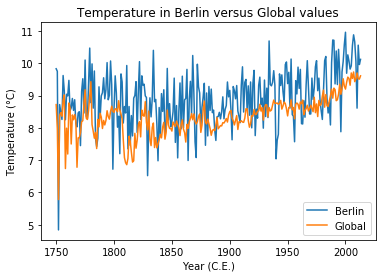
\includegraphics[width=\columnwidth]{Plots/MovingAverageTemperaturePlot_001year.png}
		% Create a subtitle for the figure.
		\caption{Average temperature in Celsius over time in years before data transformations with Berlin shown in blue and Global values shown in orange.}
		% Define the label of the figure. It's good to use 'fig:title', so you know that the label belongs to a figure.
		\label{fig1}
		\end{center}
	\end{figure}

    The average temperature in Berlin has a wider variance than the global average over time due to the global average containing various biomes with differing atmospheric properties such as pressure and chemical composition, precipitation types, latitude/longitude, altitude relative to sea level and sunlight exposure. Covering large and varied areas means that it is difficult to change the global average values. The average temperature is also driven downward relative to Berlin because it does not have icy tundras and arctic areas. However, Berlin also does not contain scorching deserts either, this means that the global average tends to have more cold places relative to Berlin than warm ones.\\

    When the data was transformed to a 7 year moving average, as can be seen by figure \ref{fig2}. The trends become more obvious because they are less obscured by sporadic fluctuation and become more consistent as they become less prone to outliers as seen with the consistent global temperatures. However, if temperatures rise uniformly then this will result in a higher average.\\

    It is well known to statisticians that the mean is a metric that is prone to outliers, this means that it could be possible to stabilise the values further by using a metric which does hot have this drawback. The mode is a metric which meets this condition as metric of central tendency which is known to be less prone to outliers making likely to be a better candidate than the mean.\\

    The same trend of Berlin having a higher temperature relative to the global average and the presence of large fluctuations in temperatures during the late 1700s is still evident. However, the exponential rise of temperature over time becomes easier to spot as the temperature rises at an accelerating rate as the years progress. This suggests that the forces which are driving climbing temperatures are compounding themselves. This could coincide with the rising carbon dioxide emissions per capita as the global population increases exponentially. However, the causal reason for the change cannot be inferred from this data alone and thus what problems rising temperatures will have and what should be done about them cannot be discussed in this analysis.\\

	\begin{figure}[tbh]
		\begin{center}
		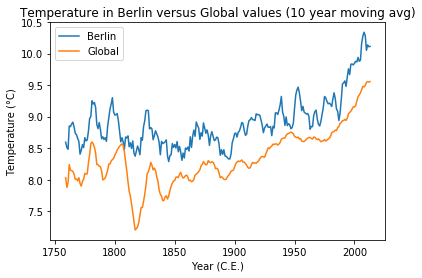
\includegraphics[width=\columnwidth]{Plots/MovingAverageTemperaturePlot_010years.png}
		\caption{Seven year moving average of the temperature in Berlin (shown in blue) against the corresponding Global values.}
		\label{fig2}
		\end{center}
	\end{figure}

    This evidence could cause for alarm because there are many systems on the planet which are dependent on temperature from atmospheric chemistry which determines the quality of air to dissolved carbon dioxide in the water, which can decrease the acidity of various bodies of water, which can then have knock on effects for aquatic life or oceanic currents. Effected organisms which are part of a large network can also propagate problems further. Hence, if the rising temperature should be a problem then it should also be able to see these effects across various scientific disciplines. It is worth noting that the rising temperature of the globe by roughly 1.5°C is not trivial and requires a large amount of energy to do as discussed earlier in this document. Hence, whatever is causing this ought to be a proportionally large process.

\section{Conclusion}
	In conclusion, there is evidence to suggest that the temperature of the globe has been rising over the past century at a rate which seems to be exponential. This could have a profound effect on global ecosystems as many of them are dependent on temperature in order to function naturally. More research is required in order to determine where this change in temperature comes from and what should be done about it if at all and what this could mean for the world.

% Your document ends here!
\end{document}
